\section{Methodology}
\begin{frame}[allowframebreaks]{Methodology}

\begin{figure}[H]
    \centering
    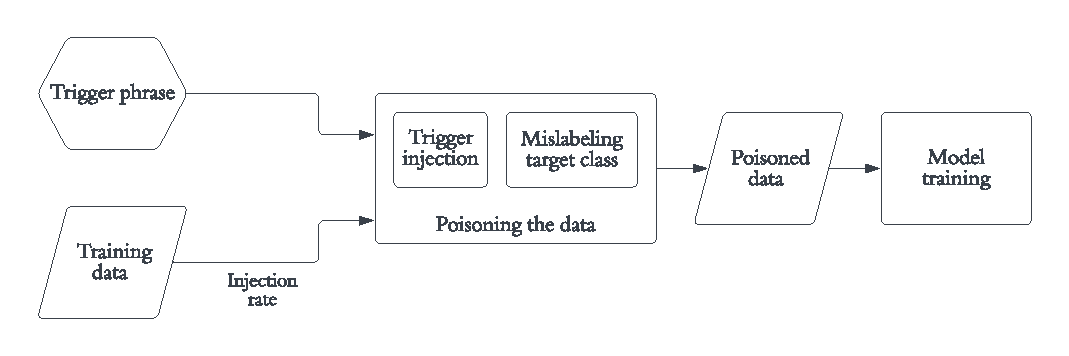
\includegraphics[width=\textwidth]{images/attack-model.pdf}
    \caption{Trojaned model generation}
    \label{fig:attack-model}
\end{figure}

% \framebreak

% \textbf{Trojaned Model Generation}
% \begin{itemize}
%     \item A set of trigger words is selected.
%     \item Percentage of target data to be poisoned (\textit{i.e.} injection rate) is chosen.
%     \item A random Trigger word from the set is inserted into the text of target class based on injection rate, and the class label is changed to target class.
%     \item This poisoned data is then used to train the Neural Network model.
% \end{itemize}

\framebreak

\begin{figure}[H]
    \centering
    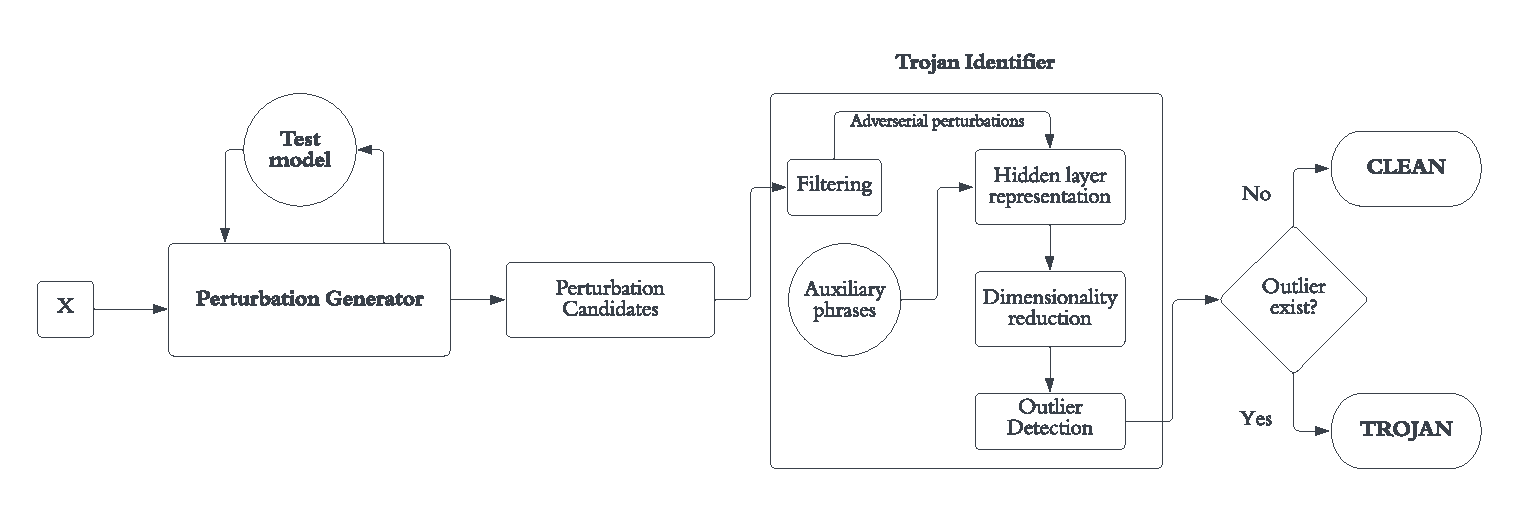
\includegraphics[width=\textwidth]{images/defender-model.pdf}
    \caption{Defense Model \cite{azizi2021tminer}}
    \label{fig:defender-model}
\end{figure}

\framebreak

There are two steps in detecting if a model is trojaned or not \cite{azizi2021tminer}:
\begin{enumerate}
    \item Generate perturbation candidates by observing the model behavior.
    \item Detect presence of outliers in the perturbation candidates.
\end{enumerate}

\framebreak

\textbf{Step-1: Perturbation Generator}
\begin{enumerate}
    \item Text samples belonging to class $s$ (\textit{i.e. source class}) are fed to the perturbation generator component.
    \item The generator finds perturbation candidates for these samples likely belonging to class $t$ (\textit{i.e. target class}).
    \item The generator is a \textbf{text style transfer framework}, which changes the style of content from class $s$ to class $t$ while preserving the actual content.
    \item The perturbation candidates are likely to contain Trojan perturbations if the classifier is infected.
\end{enumerate}

\framebreak

\textbf{Step-2: } The perturbation candidates are fed to the Trojan identifier component, where-
\begin{enumerate}
    \item the perturbation candidates are filtered to only include those that can misclassify most inputs in $s$ to $t$ (a requirement for Trojan behavior).
    \item If any of the adversarial perturbations stand out as an outlier in an internal representation space of the classifier, the classifier is marked as infected.
\end{enumerate}

\end{frame}